\documentclass[a4paper,11pt,titlepage]{article}
\usepackage[czech]{babel}
\usepackage[utf8]{inputenc}
\usepackage{latexsym}
\usepackage[dvips]{graphicx}
\pagestyle{headings}
\hyphenation{sou-sta-vy}
\author{Jan Sedlák}
\title{Uživatelský manuál k programu Tafel}
\frenchspacing
\begin{document}
\maketitle
\tableofcontents
\newpage
\section{O programu}
Program Tafel slouží k vykreslování kuželoseček do kartézské souřadné soustavy.
\subsection{Kuželosečky}
Mezi obecné kuželosečky patří kružnice, elipsa, parabola a hyperbola. Bod a přímka se dají také vyjádřit obecnou rovnicí, ale nepatří mezi obecné kuželosečky (pro naprosté objasnění problému doporučuji článek kuželosečky na české wikipedii) a program Tafel se jimi nezabývá.\\

\emph{Všechny kuželosečky se dají vyjádřit obecnou rovnicí}\\

\emph{$a*x^{2}+b*x*y+c*y^{2}+d*x+e*y+f=0$}\\

\emph{a v této obecné rovnici očekává program vstup\footnote{Vstup musí být v naprosto dopočítané obecné rovnici, program pouze pracuje s hodnotami, ale nesnaží se je nijak dopočítávat.}.}\\

Pro získání souřadnic $x$ a $y$ můžeme použít následující kvadratické rovnice (které získáme vypočítáním z obecné rovnice kuželoseček):\\

%tady je prvni vzorec
\emph{$y_{1,2}=\frac{-(b*x+e)\pm \sqrt{(b*x+e)^{2}-4*c*(d*x+f)}}{2*c}$}\\

a\\

%tady je druhy vzorec
\emph{$x_{1,2}=\frac{-(b*y+d)\pm \sqrt{(b*y+d)^{2}-4*a*(e*y+f)}}{2*a}$}\\

Idea byla taková, že po vykreslení souřadné soustavy program projede veškeré pixely ve směru osy x a poté ve směru osy y, zjistí zda-li pro daný bod existuje (popřípadě jestli je jeden, nebo dva) odpovídající bod a poté ho vykreslí. Protože pro zjištění používá předchozí rovnice, je patrné, že musí určitě být zadány hodnoty $a$ a $c$, jinak je v programu dělení nulou (to je také ten důvod, proč program nemůže vykreslovat bod a přímku). Pravda je však taková, že u některých parabol je hodnota $a$ NEBO hodnota $c$ nulová. Naštěstí není případ, že by byly nulové obě zároveň, proto vše program kontroluje a poté vykresluje jenom v ose x (popřípadě jenom v ose y). Z tohoto důvodu jsou ale některé paraboly vykreslené nedokonale (jejich vrchní části jsou pouze vytečkovány). Z důvodu chybejících hodnot $a$ a $c$ také nelze vykreslit speciální případ hyperboly, rovnoosou hyperbolu.
\newpage
\section{Kompilace programu}
Program je dle licence GNU/GPL distribuován i s kompletnímy zdrojovými kódy. Je určen pro Unix* like systémy (Linux, BSD\ldots) ale může být zkompilován i na Windows (kde je však kompilace složitější).\\

\subsection{Kompilace na Linuxu a ostatních Unix* like systémech}
Balíčkovacím systémem vaší distribuce stáhněte balíčky SDL, SDL-devel a SDL\_gfx (je možno je zkompilovat ze zdrojových kódu), v konzoli ve složce se zdrojovými kódy napište "make" a program se sám zkompiluje.\\

\subsection{Kompilace pod Windows}
Pro zkompilování balíčků pod Windows musíte mít staženy a zkompilovány knihovny SDL, SDL-devel a SDL\_gfx. Bohužel, v binární podobě jsou pro Windows k nesehnání (s obtížemi se ale sehnat dají, zkuste google) a tak jsou dvě možnosti. Buď stáhnout a zkompilovat SDL (s tím není moc velký problém, návod je na oficiálních stránkách) a SDL\_gfx (zde už je problém větší) ze zdrojových kódů, stáhnout si C++ kompiler pro Windows (MS C++ Visual Studio apod.) a zkompilovat zdrojové kódy v závislosti na zvoleném kompileru, či stáhnout si IDE jménem Dev-C++ (s kompilerem Mingw), odsud stáhnout SDL a SDL\_gfx z balíčků jako plugin (volba \uv{Získání aktualizací}) a zkompilovat poté program v něm. Hodně štěstí při kompilaci na tuto zvláštní, téměř nepoužitelnou a divně se chovající platformu.
\newpage
\section{Používání programu}
Program je napsán primárně na platformu Linux, je POSIX kompatibilní a lze ho zkompilovat také na platformu Windows. Program Tafel patří mezi konzolové programy, ač používá grafiku, hodnoty se předávají programu v konzoli a je odsud také spouštěn. Nezapomeňte, že na platformě Windows musí být soubor SDL.dll umístěn buď ve složce C:$\backslash$Windows$\backslash$System32 nebo ve složce s programem. Zapněte svůj oblíbený emulátor terminálu (gnome-terminal, terminal, konsole, xterm) popřípadě \uv{emulátor} téměř nepoužitelné příkazové řádky (ve Windows), přepněte se do složky se zkompilovanou binárkou a program spusťte (\uv{./název\_programu} v Linuxu,\\  \uv{název\_programu.exe} ve Windows). Hodnoty se (jako u všech pořádných programů) předávají programu přímo při spuštění (narozdíl od zastaralého Pascalu toto C/C++ umožňuje) a program očekává tyto argumenty:\linebreak[4]

\begin{description}
\item -a X = písmeno X nahraďte hodnotou, která má být u členu $x^{2}$
\item -b X = písmeno X nahraďte hodnotou, která má být u členu $x*y$
\item -c X = písmeno X nahraďte hodnotou, která má být u členu $y^{2}$
\item -d X = písmeno X nahraďte hodnotou, která má být u členu $x$
\item -e X = písmeno X nahraďte hodnotou, která má být u členu $y$
\item -f X = písmeno X nahraďte hodnotou absolutního členu (poslední člen bez neznámých)
\end{description}

Defaultní hodnotou všech proměnných je 0 (pokud explicitně nevyžádáte nastavení nějaké proměnné na určitou hodnotu, je automaticky nastavena na 0).\linebreak[4]

\begin{description}
\item -ec X = písmeno X nahraďte jednou s barev (red, white, green, blue, black, yellow, purple) - tuto barvu bude kuželosečka mít
\item -n = zadejte pro zadávání nové kuželosečky (když chcete vykreslit více kuželoseček na jednu 0xy)
\item -v = ukáže verzi programu
\item -h = zobrazí helpfile
\end{description}

Zavoláte-li program bez argumentů, zobrazí se krátký helpfile s nápovědou k argumentům programu.\\

Po zavolání programu se vykreslí kuželosečky podle zadaných hodnot - pokud je nějaká rovnice kuželosečky špatně zadaná a nelze vykreslit, vypíše se tento fakt na chybový výstup\footnote{Pozor! - standardní a chybový výstup na Windows se z neznámých důvodů nevypisuje do konzole ale do souborů pojmenovaných cerr.txt a cout.txt. Textový výstup programu hledejte zde - je to jenom další z důkazů o omezenosti této platformy.}.\\

Pro ukončení programu stiskněte Escape.\\

Program implicitně vytváří okno aplikace o rozměrech 800x600 pixelů, je-li Vaše rozlišení menší, můžete změnit proměnné RES\_X a RES\_Y v souboru defines.h.\\

Program nekontroluje správnost předávaných argumentů, pouze je tiše akceptuje, protože vyřešením problémů se vstupy programu a argumenty by se velikost programu ztroj- až zečtyřnásobila.\\

Poslední upozornění - program pracuje tak, že jedna jednotka je jeden pixel - chcete-li proto zobrazit kružnici s poloměrem 5 jednotek, odpovídá tomu kružnice o poloměru 5 pixelů, která je téměř nezobrazitelná. V praxi je parametr -f nastavován na desítky tisíc jednotek.\\
\newpage
\section{Ukázky z běhu}
\begin{figure}[h]
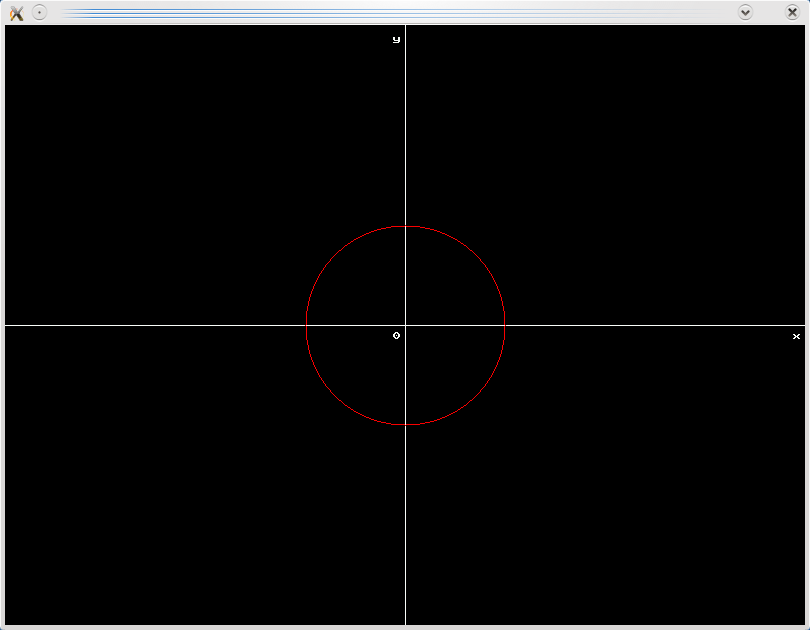
\includegraphics[width=8cm]{1.eps}\\
./tafel -a 1 -c 1 -f -10000
\end{figure}
\begin{figure}[h]
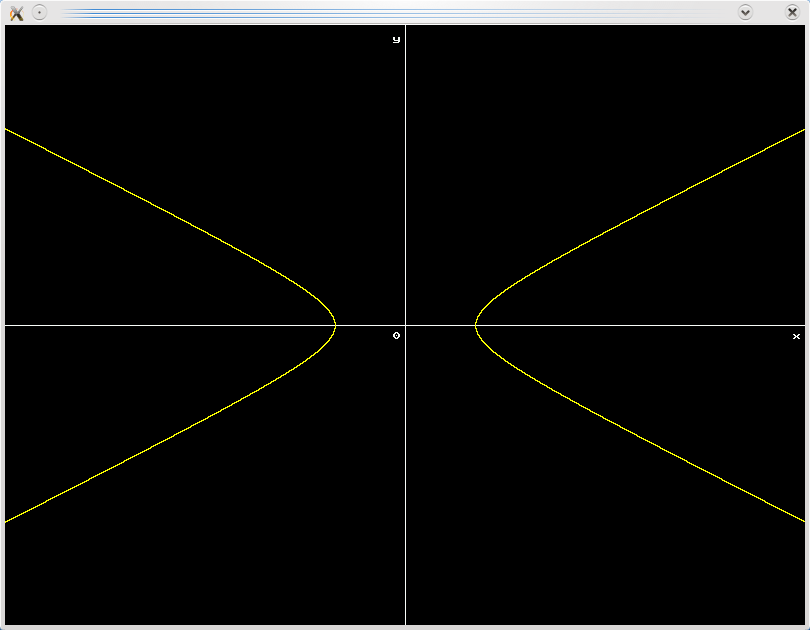
\includegraphics[width=8cm]{2.eps}\\
./tafel -a 2 -c -8 -f -10000 -ec yellow
\end{figure}
\begin{figure}[h]
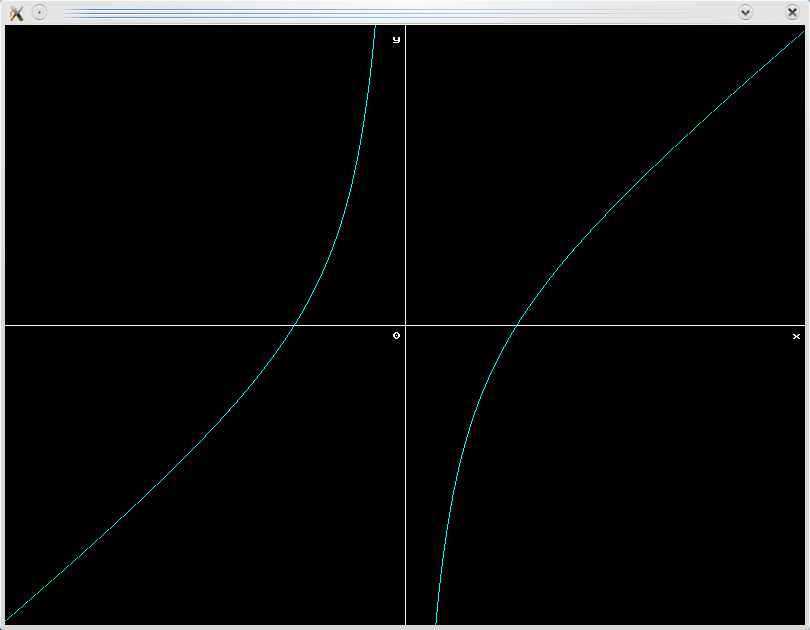
\includegraphics[width=8cm]{3.eps}\\
./tafel -a 4 -b 5 -f -50000 -ec blue
\end{figure}
\begin{figure}[h]
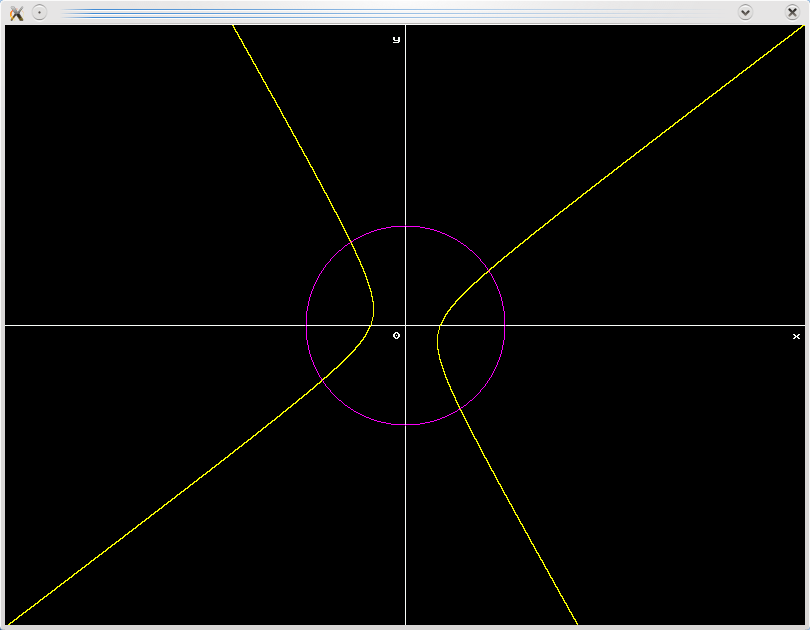
\includegraphics[width=8cm]{4.eps}\\
./tafel -a 4 -b 3 -c -3 -f -5000 -ec yellow -n -a 1 -c 1 -f -10000 -ec purple
\end{figure}
\newpage
\section{Dodatečné informace}
Program je distribuován pod licencí GNU/GPL\\
Program byl vytvořen za pomocí kompileru gcc, knihovny SDL a SDL\_gfx a byl psán v C++ v IDE Code::Blocks, Geany a vim.\\
Tento manuál byl sázen za pomocí programu \LaTeX\\

\copyright Jan Sedlák, 2009
\end{document}
